\documentclass[11pt,a4paper]{article}
\usepackage{tikz}
\usetikzlibrary{arrows.meta,positioning}
\usepackage{tabularx}
\usepackage{amsmath,amssymb,amsthm}
\usepackage{geometry}
\geometry{margin=1in}
\usepackage{hyperref}
\usepackage{graphicx}
\usepackage{setspace}
\onehalfspacing

\title{\textbf{Paper A-09: Earth Agricultural Intensification:\\ A Constraint-Driven Flux Dynamics (CDFD) Perspective}}
\author{Steve Bico Mujjabi, MD\\
\small Independent Researcher\\
\small Founder, Vura Labs\\
\small Kampala, Uganda\\
\small ORCID: 0009-0001-0556-5516}
\date{August 2026}

\begin{document}
\maketitle

% BEGIN SHARED-METHODS POINTER
\noindent\textit{Shared Part IV notation and evidence boundaries are defined in \path{PART_IV_METHODS_AND_CLAIM_BOUNDARY.md}. This paper states only its local observables, comparison, and failure conditions.}
% END SHARED-METHODS POINTER


\begin{abstract}
This paper develops a falsifiable CDFD/AFL model of Earth Agricultural Intensification. It maps fertilizer, water, energy, labor, capital, and production demand to driving flux $\Phi$, soil, water, pest, biodiversity, and infrastructure limits to active constraint $C$, crop diversity, management, storage, irrigation, and substitution to responsiveness $S$, and soil degradation, resistance, farm capital, and management history to structural memory $M_s$. The target outcome is yield, yield variance, externalities, and recovery, tested against long-term agricultural trials, yield records, soil assays, remote sensing, and input accounts. The paper treats universality as a shared model architecture rather than an assertion that unlike systems have the same material mechanism. It states the negative result that would make the mapping unnecessary and places the domain claim inside the cumulative CDFD programme and its reproducible runtime boundary.
\end{abstract}

\section{Introduction}

Agriculture is the process by which human civilization engineers the Earth's surface to maximize a specific thermodynamic output: edible biomass. A farm is a highly manipulated biological engine.

In a natural ecosystem, energy and nutrients cycle in closed loops. In industrial agriculture, the loop is severed. Humans artificially pump massive volumes of nitrogen and phosphorus into the system, and aggressively extract the resulting biomass. In CDFD terms, this is an attempt to sustain an infinite, unidirectional flux without regard for the underlying topological constraints.

\section{The Agrarian Adaptive Surface}
We apply the Adaptive Operating Ratio to a cultivated field:
\begin{equation}
    \Psi_s = \left( \frac{\Phi}{C} \right) \cdot S \cdot M_s
\end{equation}

For an industrial monoculture:
\begin{itemize}
    \item \textbf{Flux ($\Phi$)}: The agricultural yield (tons per hectare) actively extracted from the system, and the corresponding massive influx of synthetic fertilizers.
    \item \textbf{Constraint ($C$)}: The physical limitations of the soil matrix, water scarcity, and the buildup of soil salinity from chemical inputs.
    \item \textbf{Responsiveness ($S$)}: The natural fertility and microbiome biodiversity of the topsoil, which in a natural state acts to elastically buffer environmental shocks.
    \item \textbf{Memory ($M_s$)}: Ecological desertification and topsoil loss. As heavy machinery compacts the soil and chemicals kill the microbiome, the field "remembers" the trauma. The soil matrix rigidly locks into a barren, hydrophobic state.
\end{itemize}

\subsection{The Illusion of Infinite Yield}
To maximize harvest, industrial farming aggressively kills pests and weeds. In CDFD terms, this artificially forces natural constraints to zero ($C \to 0$). Simultaneously, immense synthetic flux ($\Phi$) is injected. The adaptive ratio skyrockets ($\Psi_s \gg 1$), producing an explosion of biomass.

However, this state is topologically unsustainable. The artificial inputs actively destroy the natural responsiveness $S$ (the soil microbiome). Because $S$ drops toward zero, the farmer must apply exponentially more synthetic flux $\Phi$ every year just to maintain the same yield.

Eventually, the systemic memory $M_s$ locks in. The topsoil is dead, compacted, and salinized. When a natural shock occurs (e.g., a drought), there is no biological elasticity ($S$) left to absorb it. The equation collapses ($\Psi_s \ll 1$), resulting in catastrophic crop failure (e.g., the Dust Bowl).



\section{Measurement Layer}

% BEGIN PART IV MAJOR CROSS-DOMAIN UPGRADE
\section{Cross-Domain Model Upgrade: Mechanism, Scale, and Tests}

\subsection{Observable Translation}

The paper-specific translation begins with an observable chain rather than a
verbal analogy. For Earth Agricultural Intensification, the proposed drive is fertilizer, water, energy, labor, capital, and production demand.
The active limitation is soil, water, pest, biodiversity, and infrastructure limits. Responsiveness is carried by
crop diversity, management, storage, irrigation, and substitution, while retained state is represented by
soil degradation, resistance, farm capital, and management history. The outcome to explain is yield, yield variance, externalities, and recovery.

\begin{table}[htbp]
\centering
\small
\caption{Operational CDFD/AFL map for Paper A-09.}
\begin{tabularx}{\textwidth}{|l|X|X|}
\hline
\textbf{Term} & \textbf{Paper-specific observable meaning} & \textbf{Measurement question} \\
\hline
$\Phi$ & fertilizer, water, energy, labor, capital, and production demand & What rate, load, gradient, or demand enters the focal system? \\
\hline
$C$ & soil, water, pest, biodiversity, and infrastructure limits & Which measured bottleneck limits transfer, function, or recovery? \\
\hline
$S$ & crop diversity, management, storage, irrigation, and substitution & Which process changes effective capacity or reroutes the load? \\
\hline
$M_s$ & soil degradation, resistance, farm capital, and management history & Which retained state makes equal present loads produce different futures? \\
\hline
$Y$ & yield, yield variance, externalities, and recovery & Which outcome is predicted out of sample, with uncertainty? \\
\hline
\end{tabularx}
\end{table}

\begin{figure}[htbp]
\centering
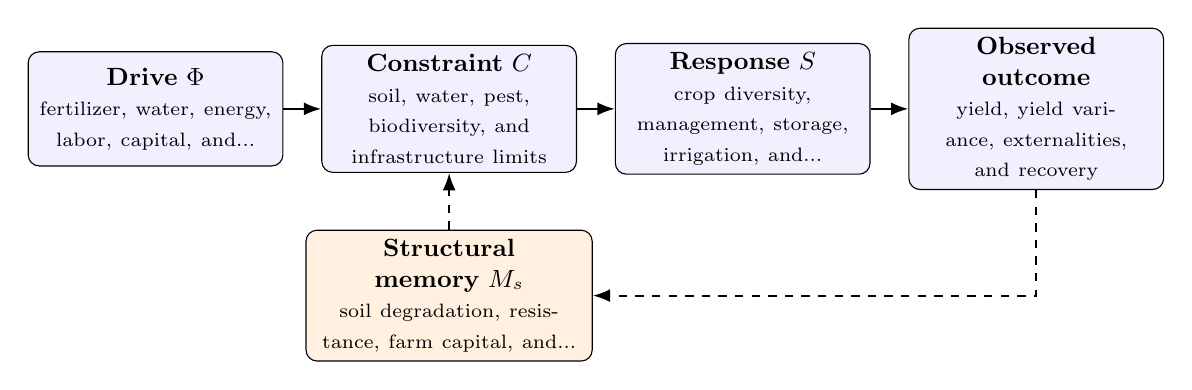
\begin{tikzpicture}[
    node distance=0.48cm,
    every node/.style={font=\small},
    box/.style={draw, rounded corners, align=center, minimum height=1.45cm, text width=3.0cm, fill=blue!6},
    memory/.style={draw, rounded corners, align=center, minimum height=1.25cm, text width=3.4cm, fill=orange!12},
    flow/.style={-{Latex[length=2.2mm]}, thick},
    feedback/.style={-{Latex[length=2.2mm]}, thick, dashed}
]
\node[box] (drive) {\textbf{Drive $\Phi$}\\\scriptsize fertilizer, water, energy, labor, capital, and...};
\node[box, right=of drive] (constraint) {\textbf{Constraint $C$}\\\scriptsize soil, water, pest, biodiversity, and infrastructure limits};
\node[box, right=of constraint] (response) {\textbf{Response $S$}\\\scriptsize crop diversity, management, storage, irrigation, and...};
\node[box, right=of response] (outcome) {\textbf{Observed outcome}\\\scriptsize yield, yield variance, externalities, and recovery};
\node[memory, below=0.72cm of constraint] (memory) {\textbf{Structural memory $M_s$}\\\scriptsize soil degradation, resistance, farm capital, and...};
\draw[flow] (drive) -- (constraint);
\draw[flow] (constraint) -- (response);
\draw[flow] (response) -- (outcome);
\draw[feedback] (outcome.south) |- (memory.east);
\draw[feedback] (memory.north) -- (constraint.south);
\end{tikzpicture}
\caption{Paper A-09 observable CDFD/AFL architecture for Earth Agricultural Intensification. Solid arrows give the proposed forward chain; dashed arrows make history-dependent feedback explicit.}
\label{fig:a09-architecture}
\end{figure}

\subsection{Paper-Specific Causal Hypothesis}

For this paper, the hypothesized causal sequence is specific. A change in
fertilizer, water, energy, labor, capital, and production demand arrives faster than crop diversity, management, storage, irrigation, and substitution can compensate.
This raises or redistributes soil, water, pest, biodiversity, and infrastructure limits. If the load persists,
the retained state encoded by soil degradation, resistance, farm capital, and management history changes the next response, so a later event of equal
magnitude can produce a different trajectory in yield, yield variance, externalities, and recovery. The
scientific task is to estimate that sequence against the best ordinary model of
the domain, not merely to redescribe the outcome after it occurs.

\subsection{Cross-Scale Translation Without Mechanistic Erasure}

For the Earth systems family, the cross-domain translation compares coupled transport, finite environmental capacity, buffering, and retained landscape or ecosystem state. It cannot erase conservation laws, geometry, or scale; it must expose where those domain equations create comparable overload and recovery structures. \cite{Holling1973,Turing1952,BakTangWiesenfeld1987}
The required scale declaration for this paper is seasons to centuries; fields to food systems. At short
scales, the key question is whether the incoming drive is transmitted,
buffered, or diverted. At intermediate scales, response changes effective
capacity and network exposure. At long scales, retained structure can alter the
state space itself. A result is genuinely cross-scale only when the aggregation
rule is stated and the same conclusion is not an artifact of averaging.

\subsection{Evidence Ladder and Discriminating Tests}

\begin{table}[htbp]
\centering
\small
\caption{Evidence ladder for Paper A-09. Each rung can fail independently.}
\begin{tabularx}{\textwidth}{|p{0.17\textwidth}|X|X|}
\hline
\textbf{Test} & \textbf{Design} & \textbf{Discriminating result} \\
\hline
Proxy audit & Measure long-term agricultural trials, yield records, soil assays, remote sensing, and input accounts and preregister how each record maps to $\Phi$, $C$, $S$, $M_s$, and $Y$. & The mapping fails if proxies are non-identifiable, circular, or change meaning across cases. \\
\hline
Load ramp & Apply or observe input intensification followed by drought or input withdrawal while estimating the dominant constraint and response time. & A threshold claim requires a reproducible nonlinear change and uncertainty bounds, not a visually chosen breakpoint. \\
\hline
Recovery and memory & Match present load across units with different histories, then compare recovery paths. & The memory claim requires history-dependent divergence after current conditions are controlled. \\
\hline
Model comparison & Compare the baseline domain model with and without the CDFD/AFL state variables using held-out data. & The paper's stated falsifier is: the framework cannot distinguish durable yield from short-lived throughput gains. \\
\hline
\end{tabularx}
\end{table}

\subsection{Research Programme and Boundary Conditions}

The immediate research programme has four steps. First, construct a documented
dataset from long-term agricultural trials, yield records, soil assays, remote sensing, and input accounts and retain raw units before normalization.
Second, fit a baseline domain model and report its calibration and out-of-sample
error. Third, add the smallest identifiable CDFD/AFL state extension and test
whether it improves prediction of yield, yield variance, externalities, and recovery. Fourth, repeat the
analysis across the declared scale range and publish negative cases as part of
the cross-domain translation audit.

% END PART IV MAJOR CROSS-DOMAIN UPGRADE

\section{Conclusion}
Industrial monoculture is the agricultural equivalent of a hyper-leveraged financial market. It maximizes short-term throughput by intentionally destroying the system's underlying topological resilience. Through CDFD, we frame the hypothesis that sustainable agriculture requires prioritizing the biological responsiveness ($S$) of the soil rather than merely maximizing the output flux ($\Phi$).
\section*{Conflict of Interest} The author declares no conflict of interest.
\section*{Data Availability}
Part-specific runtime diagnostics are under each Part's \path{outputs/} directory.

Release-wide code: \path{Part_E_Synthesis/supplementary/}.

Generated summaries: \path{Part_E_Synthesis/outputs/}.

Figures: \path{Part_E_Synthesis/figures/}.


\section{Reference Layer}
\bibliographystyle{plain}
\bibliography{universal_afl_references}
\end{document}
